
\documentclass[preprint,12pt]{elsarticle}
\usepackage{graphicx,amsmath,amssymb,amsfonts,bm}

\renewcommand{\topfraction}{0.88}
\renewcommand{\bottomfraction}{0.80}
\renewcommand{\textfraction}{0.10}
\renewcommand{\floatpagefraction}{0.80}

\begin{document}

\section{Algebraic Conditioning and Support Selection}
Some text here introducing the section and referencing Figure~\ref{fig:vnmm_singularities_matrix_A}.

\begin{figure}[!htbp]
\centering
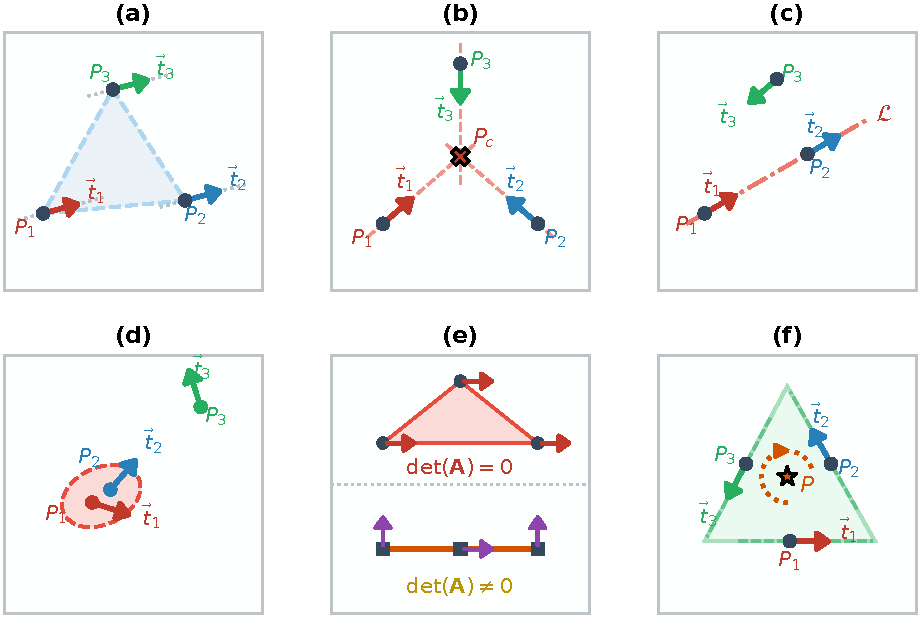
\includegraphics[width=0.80\linewidth]{artigo/figura_singularidades_matriz_A.pdf}
\caption{Geometric and directional singularity configurations of the VNMM 2D local placement matrix $\mathbf{A} \in \mathbb{R}^{3 \times 3}$ for the $\mathcal{L}^1$ solenoidal vector basis: (a) Global vector parallelism; (b) Concurrent lines of action; (c) Shared line of action; (d) Nodal coincidence; (e) Decoupling of spatial geometry and vector alignment; (f) Admissible and stable support.}
\label{fig:vnmm_singularities_matrix_A}
\end{figure}

\subsection{Singularities in L1}
To establish a systematic classification of algebraic singularities, we revisit the matrix:
\begin{equation}
\mathbf{A} = \begin{bmatrix} t_{1x} & t_{1y} & x_1 t_{1y} - y_1 t_{1x} \ t_{2x} & t_{2y} & x_2 t_{2y} - y_2 t_{2x} \ t_{3x} & t_{3y} & x_3 t_{3y} - y_3 t_{3x} \end{bmatrix}
\end{equation}
More text here to see if it fits on the same page.
\end{document}
